\section{Introduction au HPC}\label{sec:hpc_intro}


\subsection{Le calcul scientifique et la simulation numérique}
%%%%%%%%%%%%%%%%%%%%%%%%%%%%%%%%%%%%%%%%%%%%%%%%%%%%%%%%%%%%%%

    La simulation numérique est un procédé qui permet de prédire un phénomène sur un ordinateur en programmant des algorithmes mathématiques. Lorsque l'on évoque la simulation numérique, on pense souvent aux domaines physiques tel que la météorologie, la mécanique, la biologie mais elle peut aussi être appliquée en sciences humaines comme en démographie ou sociologie.La simulation numérique est aujourd'hui très utilisée car elle possède de nombreux avantages. Elle permet de réaliser des calculs dans un temps raisonnable qui ne pourraient pas être fait par un humain (prévoir la météo du lendemain). Elle permet aussi de pouvoir simuler des phénomènes dont les conditions ne sont pas reproductibles sur terre comme dans le domaine de la physique appliquée. Par exemple la théorie des cordes utilise des modèles qui n'ont pas pu être validé par aucune expérience. Un autre avantage est de réduire drastiquement les coûts d'une expérience. Par exemple pour la réalisation le crash automobile, ou ce ne sont plus de réels modèles de voiture mais bien des voitures virtuelles qui sont crashées sur des murs. L'expérimentation reste nécessaire dans la plus par des cas afin de valider les modèles mais cette approche permet de réduire leur nombre, et donc leur coût.
    
    
    A l'origine, les scientifiques observaient la nature et émettaient des théories pour expliquer leurs observations. En se basant sur ces théories ils réalisaient des expériences physiques pour les valider ou non (cf figure 1.a). Ils faisaient alors de nouvelles observations pour affiner leur théorie. Les simulations numériques sont alors apparues comme des alternatives aux expériences physiques qui étaient souvent longues et onéreuses (voir \autoref{fig:tikz_simulation}). Cette approche est largement utilisée en science pour prédire l'évolution d'un phénomène dans le temps et l'espace et de nombreux domaines y ont recours. On parle alors d'expérience in silico, terme faisant référence au silicium, matériau de base des composants informatiques. Elles sont utilisées pour faire des expériences de pensé, étudier un comportement en isolant un système de certaines physiques par exemple, qui seraient impossibles à réaliser dans des modalités traditionnelles.
    
    
    %TikZ picture
    \begin{figure}
    \begin{center}
    
    \begin{minipage}[]{.5\textwidth}
    
    \begin{tikzpicture}[->,shorten >=1pt,auto,node distance=3.8cm,   scale=0.49, every node/.style={transform shape}]
      \tikzstyle{every state}=[fill=none,draw=black,text=black,  , font=\bf]
      \tikzstyle{edge_style} = [draw=black, line width=2, ultra thick]
      \tikzstyle{node_style} = [circle,draw=blue,fill=blue!20!,font=\sffamily\Large\bfseries]
    
    
      \node[state]					    (A)                     {Nature};
      \node[state]        				(B) [below of=A]        {Observations};
      \node[state,]         		    (D) [below right of=B]  {Théorie};
      \node[state, align=left]         	(C) [below left of=B]   {Expérience\\ physique};
    
      \path
    		(A) edge [edge_style]   node {} (B)
            (B) edge [edge_style]   node {} (D)
            (C) edge [edge_style]   node {} (B)
            (D) edge [edge_style]   node {} (C);
    \end{tikzpicture}
    \end{minipage}%
    \begin{minipage}[]{.5\textwidth}
    
    \begin{tikzpicture}[->,shorten >=1pt,auto,node distance=3.8cm,   scale=0.49, every node/.style={transform shape}]
      \tikzstyle{every state}=[fill=none,draw=black,text=black,  , font=\bf]
    \tikzstyle{edge_style} = [draw=black, line width=2, ultra thick]
    \tikzstyle{node_style} = [circle,draw=blue,fill=blue!20!,font=\sffamily\Large\bfseries]
    
    
      \node[state]					(A)                    {Nature};
      \node[state]        					(B) [below of=A] {Observations};
      \node[state,]         					(D) [below right of=B] {Théorie};
      \node[state, align=left]         	(C) [below left of=B] {Expérience\\ physique};
      \node[state, align=left]        	(E) [left of=C]       {Simulation\\numérique};
    
      \path
    		(A) edge [edge_style]            node {} (B)
            (B) edge [edge_style]     node {} (D)
            (C) edge [edge_style]           node {} (B)
            (D) edge [edge_style]             node {} (C)
                  edge [edge_style, bend left]     node {} (E)
            (E) edge [edge_style, bend left]  node {} (B);
    \end{tikzpicture}
    
    
    \end{minipage}
    \end{center}
    
    
     \caption{La simulation numérique a apportée une nouvelle façon d'expérimenter les théories \cite{BSC_FIB_SCA}} 
     \label{fig:tikz_simulation}
     \end{figure}



    \subsubsection{Exemples de simulation numérique}
    %%%%%%%%%%%%%%%%%%%%%%%%%%%%%%%%%%%%%%%%%%%%%%%%
    
        Dans le domaine de la santé l'étude de la structure des protéines est primordiale.  Ces molécules qui assurent les fonctions élémentaires d'une cellule interviennent dans la majorité des processus biologiques (régulation du métabolisme, défense immunitaire). Dans ce genre de simulation le pas de temps est de l'ordre de la nanoseconde. Grâce à la simulation numérique, une meilleure compréhension de ces molécules est possible ainsi que la découverte de nouvelles. Un intérêt concret de ces études est la découverte de nouveaux médicaments ou antibiotiques. 
        Aussi des modélisations peuvent être utilisée pour analyser la propagation d'un virus comme la grippe aviaire à l'échelle mondiale pour mieux prévenir les populations\cite{CEA2007}. Cette modélisation fait intervenir plusieurs paramètres comme le lieu et la période d'incubation du virus ou encore la fréquentation et destinations des passagers des 4000 principaux aéroports mondiaux.
        
        En astrophysique la simulation numérique est aussi capitale du fait de la non-reproductibilité des expériences en laboratoire.  A l'opposé de l'exemple précédent sur les protéines elle permet d'étudier des objets aussi grands que complexes que sont le système solaire, les galaxies ou bien l'univers. La simulation permet alors de faire évoluer le système avec un pas de temps aller jusqu'au million d'année. Une équipe du CEA a pu reconstituer le passé de la galaxie Andromède en analysant les observations réalisés grâce au satellite infrarouge Sptizer\cite{Block2006a}. Après avoir mis au point le modèle adéquat et après plusieurs heures de simulation, ils ont pu déterminer qu'elle avait été percutée par une galaxie compagne il a plus de 210 millions d'années et que sa forme actuelle résultait de cet impact (voir\autoref{pic:cea_galaxy}).
    
        
        \begin{figure}
            \center
            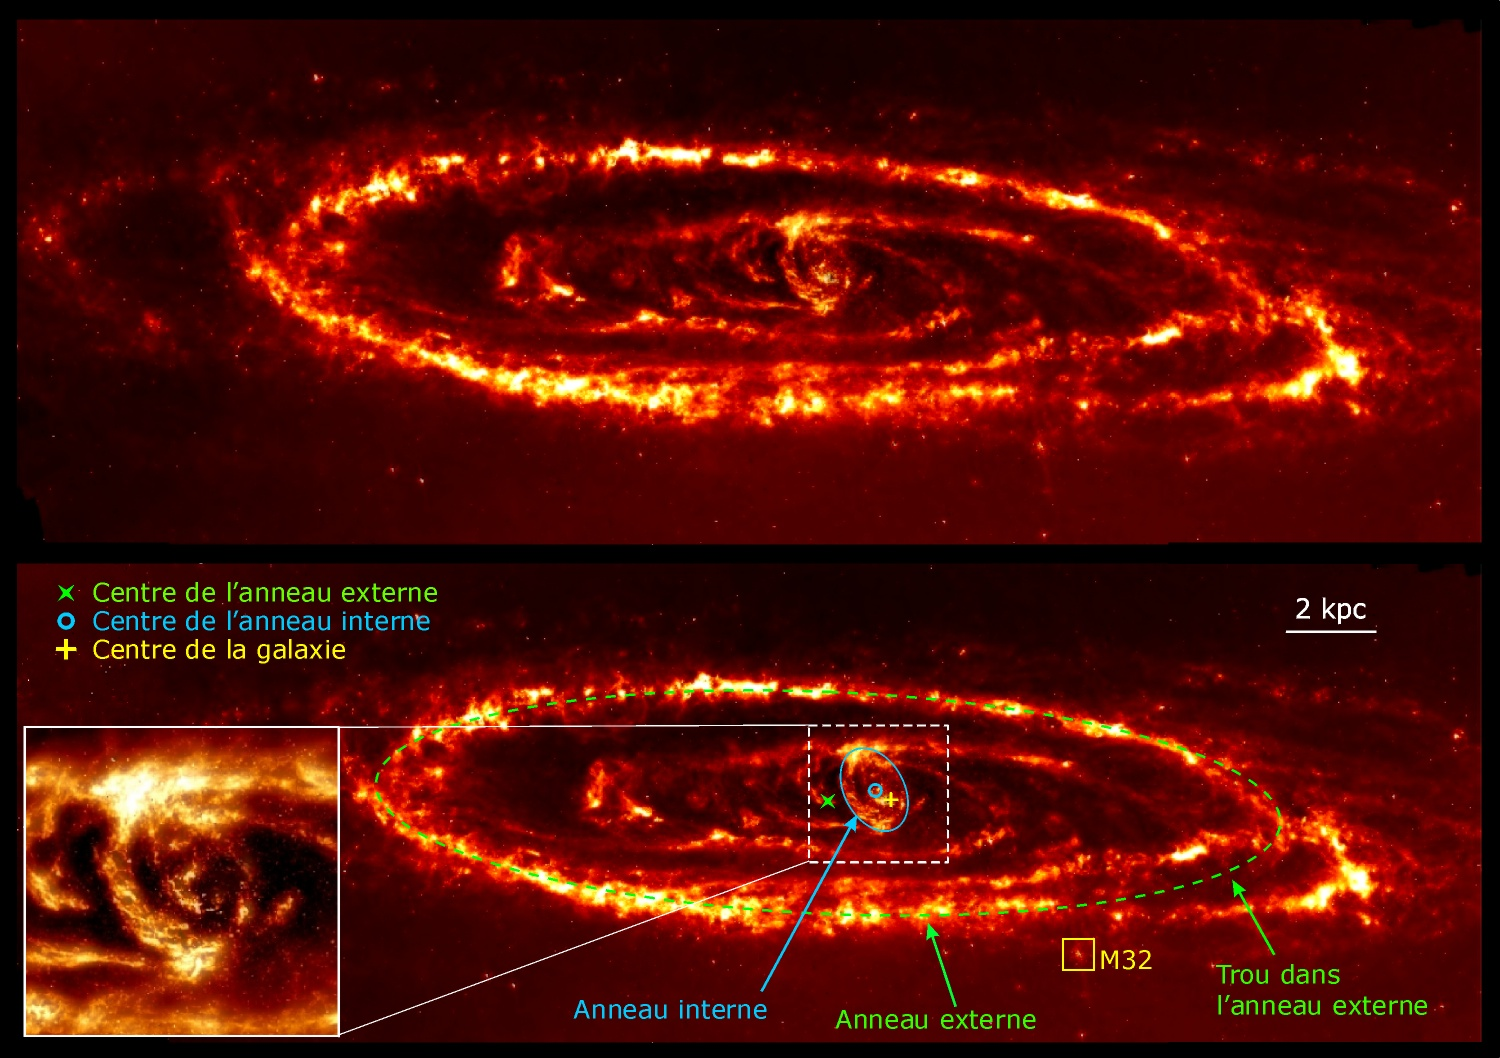
\includegraphics[width=10cm]{images/cea_galaxy.jpg}
            \caption{\label{pic:cea_galaxy} Cartographie de l'émission infrarouge des poussières  obtenue à l'aide du satellite Spitzer\protect\footnotemark. En bas : identification de la structure en double-anneau décentré et agrandissement de l'anneau interne. A la distance de M31, l'anneau interne a une dimension de 3 par 4.5 milliers d'années-lumière.}
        \end{figure}
        \footnotetext{source: \url{http://irfu.cea.fr/Phocea/Vie_des_labos/Ast/ast.php?id_ast=958&t=actu}}

    
        Dans l'industries des hydrocarbures la recherche pétrolière est très couteuse : le coût d'un forage d'exploration maritime peut atteindre les 100 millions d'euros\footnotetext{source: \url{https://www.planete-energies.com/fr/medias/decryptages/la-difficile-decision-de-lancer-un-forage}}.  Les pétroliers utilisent la simulation numérique pour analyser les fonds marins et modéliser les réservoirs de pétrole pour optimiser leur extraction. Pour cela, ils utilisent des bateaux tractant d'immenses lignes flottantes pourvues de capteurs. Le principe est d'émettre de légers ébranlements, comme une petite explosion, et d'analyser le réfléchissement des signaux sur le fond marin (voir \autoref{pic:hpl_petrole}). Grâce à l'analyse de ces données il est alors possible construire une cartographie du fond marin et ainsi déceler la présence ou non de réservoirs d'hydrocarbures.  En perçant le puit de façon optimale il sera d'autant mieux exploité. Et le risque de forer au mauvais endroit est lui aussi diminué (le taux de succès est d'un forage sur trois).

        \begin{figure}
            \center
            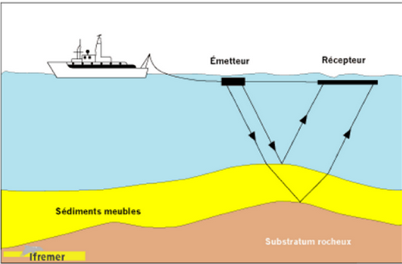
\includegraphics[width=8cm]{images/hpl_petrole.png}
            \caption{\label{pic:hpl_petrole}Étude de fond marin grâce à la sismique de réflexion.}
        \end{figure}



    \subsubsection{Méthodes de calculs}
    %%%%%%%%%%%%%%%%%%%%%%%%%%%%%%%%%%%%%%%%%%%%%%%%
    
        La majorité de ces simulations son basés sur des équations dites \textit{gouvernantes} qui sont des approximations des phénomènes étudiés. Comme les ordinateurs ne peuvent pas exécuter une infinité d'instructions, ces équations ne peuvent pas être utilisées directement et ont besoin d'être discrétisé. Pour résoudre les équations mathématiques d'un modèle il existe deux approchent principales : la méthode de calcul déterministe et la méthode de calcul statistique. 
        
        La première se base sur la discrétisation de l'objet étudié en volumes élémentaires contigus. En mathématiques, la discrétisation est un procédé qui permet de passer d'une fonction ou d'un modèle à son équivalent continu (\autoref{pic_maillage}). Ce procédé ne permet pas de décrire le phénomène réel, mais de l'approximer avec plus ou moins d'erreur. Pour améliorer ces simulations, ces représentations doivent utiliser des maillages le plus fin possible en tenant compte des problèmes de stabilité mathématique. C'est en cela que ces simulations nécessitent d'énormes puissances de calculs.
        La deuxième approche utilise des modèles probabilistes pour représenter un comportement. Elle est adaptée pour des phénomènes ou chaque élément peut subir différents événements. Pour chaque étape du calcul, l'objet évolue grâce à des tirages aléatoires (méthode de Monte Carlo \cite{Kroese2014}). 
        
                 
        \begin{figure}
        \center
        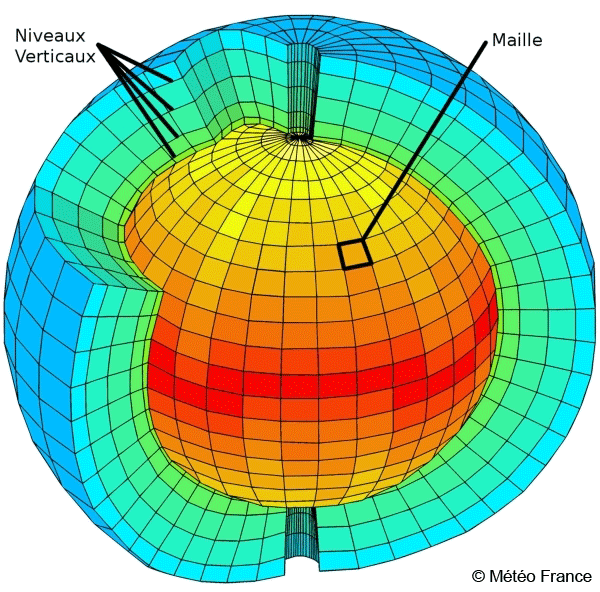
\includegraphics[width=5cm]{images/Chapitre1/maillage.png}
        \caption{\label{pic_maillage} Le maillage le plus fin exploité par Météo-France pour ses prévisions régionales restitue des mailles de 2,5 km de côté (source \url{www.irma-grenoble.com}).}
        \end{figure}
      
  
    \subsubsection{Lien entre simulation et HPC}
    %%%%%%%%%%%%%%%%%%%%%%%%%%%%%%%%%%%%%%%%%%%%%%%%
    
        Si la simulation numérique est très utilisée depuis ces 30 dernières années cela ne veux pas dire qu'elle n'existait pas avant. En effet des scientifiques comme Pythagore réalisés ces simulations en faisant des calculs manuels ou en s'aidant de tables déjà pré-calculées. Du fait de la limitation de leur capacité de calcul et de temps disponible, c'est avec l'apparition de l'informatique que les simulations sont devenus réellement exploitables.

        La majorité des domaines utilisant des simulations numériques ont un besoin insatiable de puissance de calcul. Ces simulations doivent être toujours plus précises et pouvant être réalisée sur des modèles toujours plus grand. Pour l'exemple de la météo, les météorologues voudront utiliser des simulations plus précises (réduire la taille des mailles) et pouvoir les réaliser sur de plus grands jeux de données (surface d'un pays, continent ou du globe terrestre).
        Pour améliorer ces simulations, ces représentations doivent utiliser des maillages le plus fin possible. C'est en cela que ces simulations nécessitent d'énormes puissances de calculs et que cette demande est illimité car les maillages pourront toujours être affinés. 
        
        Les domaines qui ont recours au \gls{hpc} sont nombreux notamment à travers la simulation numérique qui devient un levier d'action essentiel pour beaucoup d'industries. Pour la compétitivité et l'innovation des entreprises, les simulations numériques sont désormais un outil indispensable d'aide à la conception, à la décision et au contrôle de leurs activités. Le schéma \ref{fig:tikz_simulation} montre comment la simulation numérique est venue révolutionner de nombreux domaines scientifiques.



\subsection{Le calcul haute performance}
%%%%%%%%%%%%%%%%%%%%%%%%%%%%%%%%%%%%%%%%%%%%%%%%%%%%%%%%%%%%%%

    Que ce soit quand on consulte la météo, quand on prend sa voiture ou que l’on consomme un médicament nous utilisons un produit de la simulation numérique. Ces simulations sont des programmes informatiques qui nécessitent beaucoup de calcul, les rendant impossibles à réaliser par un être humain. La rapidité de leur exécution dépend alors de la puissance de calcul disponible pour exécuter l’application. Cette infrastructure qui en résulte est appelée un supercalculateur et le domaine qui regroupes toutes ces notions est appelé Calcul Haute Performance (HPC). Le HPC est un domaine peu connu qui pourtant impact notre vie quotidienne. Le domaine du HPC est le domaine informatique qui consiste à exécuter des applications le plus efficacement possible sur une architecture. Une telle architecture peut aller d'un simple ordinateur personnel à un centre de calculs dédié. Les plus puissantes d'entre elles appelés supercalculateur (ou \textit{cluster}) sont présentés dans la \autoref{sec:supercomputer}. 
    
    Aujourd’hui, presque que tout ce que nous utilisons a eu un jour étais simulé sur un supercalculateur à un tel point que l’avancée de nos sociétés est dépendante de la puissance de calcul disponible pour réaliser ces simulations. Le calcul haute performance est un levier essentiel de l'évolution de notre société. Dans le domaine de la santé, le \textit{Living Heart Project}\cite{Baillargeon2014} a pour objectif de modéliser un coeur pour aider à comprendre son fonctionnement et mieux prévenir les accident cardio vasculaire. Pour cela, un coeur a été modélisé et peut être étudié pour comprendre ses réactions à différent traitements. Le modèle est composé 7.500.000 éléments finis et utilisent 250.000.000 variables pour chacune des étapes de la modélisation (plus d'un millions d'étapes). Grâce aux HPC, il est possible de tester un traitement sur un patient avant de lui administrer. Ce modèle est accessible aux fabricant de matériels médicaux depuis 2017. 

    

   
    \subsubsection{Utilisateurs de HPC}
    %%%%%%%%%%%%%%%%%%%%%%%%%%%%%%%%%%%%%%%%%%%%%%%%%%%%%%%%%%%%%%
    
        Les principaux utilisateurs ayant recours au calcul haute performance peuvent être regroupé selon ces trois catégories en fonction de leur budget et de leur utilisation. La première regroupe les utilisateurs avec les plus petits budgets comme des équipes d'ingénieurs ou des petites universités qui ont besoin d'une ressource de calcul. On pourra citer le projet SIMSEO \cite{Saguez2016} qui à pour but de sensibiliser et d'accompagner les PME à utiliser la simulation numérique. Car même pour des entreprises de tailles réduite, la simulation et le HPC peuvent être des atouts clefs dans leur stratégie.
        La deuxième catégorie regroupe les grandes universités qui partagent le matériel entre plusieurs écoles ou laboratoires de recherche. Ces systèmes sont d'une puissance élevée, et certains sont classé dans le classement du \textit{TOP500} (voir \autoref{sec:top500}). La dernière catégorie d'utilisateur concerne les entreprises privées qui utilisent le calcul haute performance pour développeur leur activité (recherche et développement). Ces architectures sont les plus puissante de la planète et ne sont pas toujours listé dans le classement du Top500 par soucis de confidentialité. 
        
        
    \subsubsection{Les moyens d'accès au HPC}
    %%%%%%%%%%%%%%%%%%%%%%%%%%%%%%%%%%%%%%%%%%%%%%%%%%%%%%%%%%%%%%%%
    
        Les utilisateurs des différentes catégories listés précédemment accèdent au HPC par différents moyens:
        \begin{enumerate}
            
            \item \textbf{Le supercalculateur dédié} \textit{dedicated supercomputer}) consiste à la création d'une architecture unique qui ne sera pas répliquer. L'objectif de ce type d'infrastructure est d'être parfaitement adapté aux besoins de l'application. La conception de ces architectures étant unique, les frais de conception sont très élevés mais cette spécificité en fait des architectures très performantes. 
            
            \item \textbf{Le commodity cluster} agrège du matériel grand public (haut de gamme) pour former des grappes de calculs de plusieurs milliers de processeurs. La performance de ces architectures ne repose pas sur l'utilisation de matériels ultra-optimisés mais sur l'agrégation de centaines de noeuds travaillant ensemble. Ce modèle de supercalculateur est le plus répendu actuellement et est présenté dans la section \autoref{sec:supercomputer}.  
            
            \item \textbf{L'informatique en nuage} (\textit{cloud computing}),  utilise le modèle \textit{System as a Service} pour apporter aux entreprises manquant de moyens ou de compétences un accès à une infrastructure HPC externalisé. Les principaux avantages sont la flexibilité d'usage (adapter l'infrastructure à son besoin) ainsi que l'externalisation de la gestion de la plate-forme. L'informatique en nuage permet aussi de faciliter les évolutions de matériels et permet d'utiliser les dernières technologies. Le \textit{nuage} peut être implémenté de deux façons. La première est d'utiliser un nuage public où les machines sont gérées par le prestataire directement dans leur centre de données. La deuxième est d'installer un \textit{nuage} privé, ou le client choisi ou installer la plateforme. Cette seconde solution est particulièrement recherché par les entreprises utilisant des données sensibles et refusant qu'elles soient stockées dans un autre pays. 
            
            
        \item \textbf{Les grilles informatiques} (\textit{Grid Computing} sont un regroupement de ressources informatique à grande échelle (nationale voir internationale). Par exemple \textit{Einstein@Home} \cite{PhysRevD.80.042003} est un projet de recherche mondial sur les ondes gravitationnelles  qui regroupe les ordinateurs de 50000 utilisateurs connectés à travers le monde qui sont utilisés pour  analyser les données transcrite par des capteurs.
        \end{enumerate}
    
        
        \subsubsection{HPC ou HTC}
        %%%%%%%%%%%%%%%%%%%%%%%%%%%%%%%%%%%%%%%%%%%%%%%%%%%%%%%%%%%%%%
            
            Aujourd'hui le domaine des supercalculateurs est souvent désigné par le terme HPC, mais il y a quelques précision à apporter quant à la mauvaise utilisation de ce terme. Il existe un autre domaine qui utilise les supercalculateur, le High Throughput Computing (HTC). En effet, la communauté à voulu donner un nom aux architectures capables d'exécuter différentes applications simultanément et ce sans interruptions sur plusieurs mois. Contrairement aux applications HPC qui exécutent des taches très dépendantes les unes des autres, les applications HTC se focalisent sur l'exécution des plusieurs tâches en parallèles et assure la disponibilité maximale du nombre de ressources dont dispose le supercalculateur. Prenons pour exemple un cluster de calcul partagé dans une université. L'objectif de cette machine n'est pas d'exécuter une application toute l'année, mais plutôt de répartir le matériel disponible entre les utilisateurs pour que tous puissent l'utiliser au maximum. Une majorité des clusters d'aujourd'hui fonctionnent sur le même modèle et l'utilisation de l'expression HPC pour les désigner est en fait un abus de langage.


        \subsubsection{Exemples d'applications}
        %%%%%%%%%%%%%%%%%%%%%%%%%%%%%%%%%%%%%%%%%%%%%%%%%%%%%%%%%%%%%%

       
            Ce qui rend le HPC populaire est son large champ d’application qui s’étend des simulations numériques à l’analyse de grands jeux de données.  De telle infrastructures sont utilisées dans de nombreux domaines dont les principaux sont la simulation numérique, la cryptographie, le Big Data et l’Intelligence Artificielle. Pour la compétitivité et l'innovation des entreprises, le HPC est désormais un outil indispensable d'aide à la conception, à la décision et au contrôle de leurs activités.
            
            Les super-calculateurs ont aussi une rôle à jouer dans la sécurité nationale. Alan Turing a développé les premiers ordinateurs à cet effet lors de la fin de la deuxième guerre mondiale pour aider au décryptage des messages allemands. Aujourd’hui les super-calculateurs sont aussi associés à la compétitivité économique et les pays se sont lancé dans la course de l’Exascale de la même façon que pour la conquête de la lune. lol. Voir la liste des projets \cite{Reed2015}.







  
        
    
  
 







